%%%%% Základní nastavení pro jednostranný tisk:
%%%%% ----------------------------------------------------
% Okraje: levý 40mm, pravý 25mm, horní a dolní 25mm (ale pozor, LaTeX si sám přidává 1in)
\documentclass[12pt, a4paper]{report}
\usepackage{geometry}
\setlength\textwidth{145mm}
\setlength\textheight{247mm}
\setlength\oddsidemargin{15mm}
\setlength\evensidemargin{15mm}
\setlength\topmargin{0mm}
\setlength\headsep{0mm}
\setlength\headheight{0mm}
% \openright zařídí, aby následující text začínal na pravé straně knihy
\newcommand{\openright}{\clearpage}


%%%%% Základní nastavení pro oboustranný tisk:
%%%%% ----------------------------------------------------
% \documentclass[12pt, a4paper, twoside, openright]{report}
% \setlength\textwidth{145mm}
% \setlength\textheight{247mm}
% \setlength\oddsidemargin{15mm}
% \setlength\evensidemargin{0mm}
% \setlength\topmargin{0mm}
% \setlength\headsep{0mm}
% \setlength\headheight{0mm}
% \let\openright=\cleardoublepage


%%%%% Nastavení kódování vstupních souborů: UTF-8
%%%%% ---------------------------------------------------------------
\usepackage[utf8]{inputenc}


%%%%% Nastavení češtiny (slovenština analogicky)
%%%%% ---------------------------------------------------------------

%%% Existují dvě hlavní možnosti, jak zacházet s češtinou. Je zapotřebí zvolit právě jednu.
%%%

%%% MOŽNOST 1 (doporučujeme):
%%% * použití balíčku czech
%%%   (mimo jiné již obsahuje příkaz \uv pro sazbu českých uvozovek)
%%% * kompilace musí následně probíhat pomocí CSLaTeXu (příkaz
%%%   cslatex, resp. cspdflatex)
% \usepackage{czech}

%%% MOŽNOST 2: (zde zakomentovaná)
%%% * použití balíčku babel s volbou pro češtinu
%%% * kompilace následně probíhá standardním LaTeXem (příkaz latex,
%%% resp. pdflatex)
\usepackage[czech]{babel}
\ifx\uv\undefined\newcommand{\uv}[1]{,,#1``}\fi
%%% příkaz pro sazbu českých/slovenských uvozovek
%%% (v novějších verzích babelu je již k dispozici, stejně tak je již
%%% k dispozici v balíčku czech)


%%% Další užitečné balíčky (jsou součástí běžných distribucí LaTeXu)
%%% ----------------------------------------------------------------
\usepackage{amsmath}                %%% rozšíření pro sazbu matematiky
\usepackage{amsfonts}               %%% matematické fonty
\usepackage{amsthm}                 %%% sazba vět, definic apod.
\usepackage{bm}                     %%% tučné symboly (příkaz \bm)
\usepackage{graphicx}               %%% vkládání obrázků
\usepackage{psfrag}                 %%% dodatečná úprava popisků v postscriptových obrázcích
\usepackage{fancyvrb}               %%% vylepšené prostředí pro strojové písmo
\usepackage{natbib}                 %%% zajištuje možnost odkazovat na reference stylem AUTOR (ROK), resp. AUTOR [ČÍSLO]
\usepackage{tikz}                   %%% vkládání vektorových obrázků
\usepackage{bbding}                 %%% balíček s nejrůznějšími symboly
\usepackage{icomma}                 %%% inteligetní čárka v matematickém módu
\usepackage{dcolumn}                %%% lepší zarovnání sloupců v tabulkách
\usepackage{booktabs}               %%% lepší vodorovné linky v tabulkách
\usepackage{paralist}               %%% lepší enumerate a itemize
\usepackage{indentfirst}            %%% zaveď odsazení 1. odstavce
\usepackage[nottoc]{tocbibind}      %%% zajistí přidání seznamu literatury, obrázků a tabulek do obsahu
\usepackage[unicode]{hyperref}      %%% zajištuje generování hyperodkazů, bookmarků atp.
\hypersetup{pdftitle=Webové řešení na prodej vstupenek s~rezervací míst,
    pdfauthor=Filip Ditrich
    ps2pdf,
    colorlinks=false,               %% hyperlinky budou označeny červenými rámečky, které budou neviditelné při tisku na papír
    urlcolor=blue,
    pdfstartview=FitH,
    pdfpagemode=UseOutlines,
    pdfnewwindow,
    breaklinks                      %% zajistí, aby se dlouhé hyperodkazy mohly lámat přes více řádků
}
\usepackage{titlesec}
\titlespacing*{\chapter}{0pt}{-10mm}{5mm}
\titleformat{\chapter}{\normalfont\huge\bfseries}{\thechapter}{1em}{}


%%% Příkazy zjednodušující přenositelnost
%%% -------------------------------------
\newcommand{\FIGDIR}{./figures}    %%% cesta do adresare s obrazky


%%% Seznam použité literatury
%%% Příkaz \bibliographystyle určuje, jakým stylem budou citovány
%%% odkazy v textu, a podle jakého stylu se automaticky vygeneruje
%%% seznam literatury. V závorce je název zvoleného .bst souboru.
%%% Styly plainnat a unsrt jsou standardní součástí latexových
%%% distribucí. Styl czplainnat vyžaduje přítomnost souboru
%%% czplainnat.bst ve stejném direktoráři, v němž se nachází
%%% kompilovaná práce.
%%%
%%% Seznam literatury se vytváří na konci práce příkazem \bibliography, kde v závorce
%%% uvádíme název databázového bib souboru.
%%%
%%%
\bibliographystyle{czplainnat}    %% Autor (rok) s českými spojkami
%\bibliographystyle{plainnat}     %% Autor (rok) s anglickými spojkami
%\bibliographystyle{unsrt}        %% [číslo]

\renewcommand{\bibname}{Seznam použité literatury}


%%%%% Použití fancyvrb (fancy verbatim) při definici prostředí pro
%%%%% sazbu kódu, resp. výstupů z počítačových programů
%%%%% ------------------------------------------------------------
\DefineVerbatimEnvironment{PCinout}{Verbatim}{fontsize=\small, frame=single}


%%%%% Hlavní část dokumentu
%%%%% ---------------------
\begin{document}
%%% titulní strana
    %%%
%%%  TITULNÍ STRANA
%%%
%%%  * soubor obsahující titulní stranu bakalářské práce
%%%
%%%  ===========================================================================
\pagestyle{empty}
\begin{center}

%%% název školy
{\bfseries\large UNICORN VYSOKÁ ŠKOLA s.r.o.}

    \vspace{5mm}

    %%% název oboru
    {\Large Softwarový vývoj}

    \vfill
    \vspace{5mm}

    %%% logo školy
    \centerline{\mbox{
\includegraphics[width=83.3mm]{\FIGDIR/uu-icon}}}

    \vfill
    \vspace{5mm}

    %%% typ práce
    {\large\MakeUppercase{Bakalářská práce}}

    \vspace{15mm}

    %%% název práce
    {\LARGE\bfseries Webové řešení na prodej vstupenek s~rezervací míst}

    \vfill

    %%% autor a vedoucí práce
    \begin{tabular}{rl}
        Autor bakalářské práce:   & Filip Ditrich              \\
        \noalign{\vspace{2mm}}
        Vedoucí bakalářské práce: & Ing.\ Marek Beránek, Ph.D. \\
    \end{tabular}

    \vfill

    %%% rok
    Praha 2023

\end{center}

%%% TODO: kopie zadání
%%% čestné prohlášení
    %%%
%%%  ČESTNÉ PROHLÁŠENÍ
%%%
%%%  * soubor obsahující čestné prohlášení k bakalářské práci
%%%
%%%  ===========================================================================
\newpage
\pagestyle{empty}
\vspace*{\stretch{8}}

%%% nadpis
\noindent
{\large\bfseries Čestné prohlášení}\\

%%% text
\noindent
Prohlašuji, že jsem svou bakalářskou práci na~téma \textit{Webové řešení na prodej vstupenek s~rezervací míst} vypracoval samostatně pod~vedením vedoucího bakalářské práce a s~použitím výhradně odborné literatury a~dalších informačních zdrojů, které jsou v práci všechny citovány a~jsou také uvedeny v~seznamu použitých zdrojů.\\

\noindent
Jako autor této bakalářské práce dále prohlašuji, že v~souvislosti s~jejím vytvořením jsem neporušil autorská práva třetích osob a~jsem si plně vědom následků porušení ustanovení § 11 a následujících autorského zákona č.~121/2000~Sb.\\

\noindent
Dále prohlašuji, že odevzdaná tištěná verze bakalářské práce je shodná s~verzí, která byla odevzdána elektronicky.

%%% podpis - místo/den
\vspace{18mm}
\noindent
V \makebox[4cm]{\dotfill} dne \makebox[2.5cm]{\dotfill}
\hspace*{\fill}
\makebox[4cm]{\dotfill}

%%% podpis
\begin{flushright}
    \noindent
    Filip Ditrich
\end{flushright}

%%% poděkování
    %%%
%%%  PODĚKOVÁNÍ
%%%
%%%  * soubor obsahující poděkování za pomoc při vytvoření bakalářské práce
%%%
%%%  ===========================================================================
\newpage
\pagestyle{empty}
\vspace*{\stretch{8}}

%%% nadpis
\noindent
{\large\bfseries Poděkování}\\

%%% TODO: text
\noindent
Rád bych touto cestou srdečně poděkoval vedoucímu bakalářské práce Ing.~Markovi Beránkovi,~Ph.D.
za~čas věnovaný vedením této práce, za~příjemnou spolupráci a~za cenné poskytnuté rady a připomínky.

%%% první stránka
    %%%
%%%  PRVNÍ STRANA
%%%
%%%  * soubor obsahující první stranu bakalářské práce
%%%
%%%  ===========================================================================
\newpage
\pagestyle{plain}

%%% začátek stránkování
\setcounter{page}{6}

%%% nastavení speciálních okrajů
\newgeometry{textwidth=100mm, textheight=247mm, left=40.4mm, right=75mm}

%%% pozadí
\tikz[remember picture,overlay]
\node[opacity=1,inner sep=0pt] at (current page.center)
    {
\includegraphics[width=\paperwidth,height=\paperheight]{\FIGDIR/side-banner}};

\begin{center}

    %%% logo školy
    \centerline{\mbox{
\includegraphics[width=39.6mm]{\FIGDIR/uu-icon}}}

    \vfill

    %%% název práce v češtině
    \Large\textbf{Webové řešení na prodej vstupenek s~rezervací míst}

    \vspace{5mm}

    %%% název práce v angličtině
    \Large{Web-based ticketing solution with seat reservation}

    \vfill

    %%% logo školy
    \centerline{\mbox{
\includegraphics[width=45mm]{\FIGDIR/uu-logo}}}

\end{center}
\restoregeometry

%%% abstrakt
    %%%
%%%  ABSTRAKT
%%%
%%%  * soubor obsahující abstrakt bakalářské práce
%%%
%%%  ===========================================================================
\newpage
\pagestyle{plain}

%%% abstrakt česky
\vbox to 0.5\vsize{
    \setlength\parindent{0mm}
    \setlength\parskip{5mm}

    %%% nadpis
    {\large\bfseries TODO: Abstrakt}

    %%% TODO: text abstrakt až po dopsání práce (lol)
    \noindent
    Tato bakalářská práce se zaměřuje na vývoj frontendové části webové aplikace pro prodej vstupenek s rezervací míst. Cílem práce je vyvinout prototyp aplikace, která potenciálnímu zákazníkovi umožní zobrazit mapu míst, vybrat si preferované místo, přidat vstupenky do nákupního košíku a následně vytvořit objednávku.

    Teoretická část práce se zaměřuje na obecnou problematiku prodeje vstupenek a moderního řešení pomocí platforem a služeb poskytujících online prodej vstupenek s možností rezervací míst. Tato část dále analyzuje trh současných poskytovatelů a definuje nejhlavnější technické problémy, které mohou při vývoji takového systému vzniknout a to výhradně z pohledu frontendu.

    Praktická část práce definuje rozsah implementované aplikace, podrobně popisuje hlavní funkce, komponenty, datové modely i některé nezbytné backendové části. Kapitola o návrhu uživatelského rozhraní popisuje principy, vzory a osvědčené postupy návrhu uživatelského rozhraní v kontextu vyvíjené aplikace. Kapitola o vývoji frontendové části poté podrobně popisuje technologie, nástroje a knihovny použité při vývoji aplikace.


    \vss}

%%% abstrakt anglicky
\nobreak\vbox to 0.49\vsize{
    \setlength\parindent{0mm}
    \setlength\parskip{5mm}

    %%% nadpis
    {\large\bfseries TODO: Abstract}

    %%% TODO: text anglicky
    \noindent
    This bachelor thesis deals with the implementation of a ticketing solution using seat reservations. The aim of
    the theoretical part of the thesis is to elaborate this issue and identify the main technical challenges and requirements for the implementation
    of such a system, especially from the frontend perspective. These challenges, such as intuitive user interface, availability of information
    real-time sales information, administration and management of seating plans or final booking and payment of orders, will be discussed in this thesis
    will be described in this thesis and options for their solution will be presented. The practical part will focus on the implementation of the part of the web application dealing with
    rendering of the interactive seating plan and its interaction with the customer. In this part the user interface design will be presented
    together with an introduction of the selected technologies to be implemented. Emphasis will be placed on the optimized design of the seating plan, the specification of
    of its data format, communcation with the API and overall documentation of the components used in the resulting application. The aim of this work is to describe
    the issues and challenges in implementing a web application addressing seat ticketing and present part of a real solution for such a
    application especially from the perspective of an interactive seat selection plan.

    Keywords: interactive seating plan, seat reservations, tickets, web applications, JavaScript, React, SVG
    \vss}


%%% obsah
    \newpage
    \openright
    \tableofcontents
%%% jednotlivé kapitoly
    %%%%% Úvod
%%%%% ------------------------------------------------------------
\chapter*{Úvod}
\addcontentsline{toc}{chapter}{Úvod}

%%% Sekce - Prodej vstupenek
%%%%% Wording: ✅
%%%%% Styling: ✅
%%%%% References: ✅
%%%%% Grammar: ✅
%%% --------------------------------------------------------------
\section*{Prodej vstupenek}
\addcontentsline{toc}{section}{Prodej vstupenek}
\label{sec:uvod-prodej-vstupenek}
Prodej vstupenek na kulturní a jiné různé události je důležitou součástí zábavního průmyslu, neboť poskytuje lidem přístup na koncerty, divadelní představení, sportovní či jiné události.
Prodej vstupenek umožňuje pořadatelům těchto akcí nejen kontrolovaný průběh akce, ale především generuje dostatečný finanční tok peněz před konáním jejich akce.
Tyto finance zpravidla potřebují pro zajištění všech potřebných prostředků pro uspořádání akce a pro pořadatele se tedy jedná o jeden z klíčových faktorů úspěchu konání akce.
Potřebují tedy pro zákazníky zajistit co nejsnadnější a nejpříjemnější možnost nákupu vstupenek.

S nástupem moderních technologií se online prodej vstupenek proměnil v atraktivní a preferovaný způsob jejich nákupu, jelikož zákazníkům umožňuje snadný, pohodlný, a hlavně rychlý způsob platby, aniž by se museli kamkoliv fyzicky dostavit.
Tento nový moderní způsob prodeje vstupenek však nabízí výhody nejen zákazníkům, ale také pořadatelům akcí.
Systémy, které jsou na tomto způsobu prodeje vstupenek založeny, pořadatelům akcí umožňují bezproblémový prodej vstupenek, což vede k efektivnějšímu plánování a řízení akcí.
Tyto systémy pořadatelům také nabízejí cenné údaje o zákaznících, jejich preferencích a chování, které mohou využít při plánování marketingových strategií, cílených reklam či propagačních akcí za účelem zvýšení zapojení zákazníků a podpoření prodeje.

Jedním z nejvýznamnějších pokroků v této oblasti online řešení prodeje vstupenek bylo rozšíření o možnost rezervace míst v prostoru konání akce.
Toto řešení nově zákazníkům umožňuje zarezervovat si místo na dané události, což opět přináší několik výhod pro zákazníky, ale také pro pořadatele akcí.
Zákazníkům umožňuje rezervaci a výběr místa, které je pro ně nejvhodnější.
Pořadatelům akcí pak rezervace míst umožňuje předem plánovat kapacitu dané akce a také zjistit, jaké místo je pro zákazníky nejvíce preferované.
Dále také značně snižuje počet možných podvodů se vstupenkami, jelikož kapacita je jasně dána počtem míst k sezení a nelze ji snadno překročit.

Webová řešení prodeje vstupenek s rezervací míst se v posledních letech stávají stále více oblíbenými a využívanými v různých odvětvích, včetně zábavního průmyslu, sportu či cestování, jak je mj.\ možné vidět na grafu na obrázku~\ref{fig:polaris-market-research} znázorňujícího průzkum trhu v oblasti poskytování online systémů prodeje vstupenek.

\begin{figure}[H]
    \centering
    \caption{Graf zobrazující podíl zemí na trhu poskytování online systémů prodeje vstupenek.}
    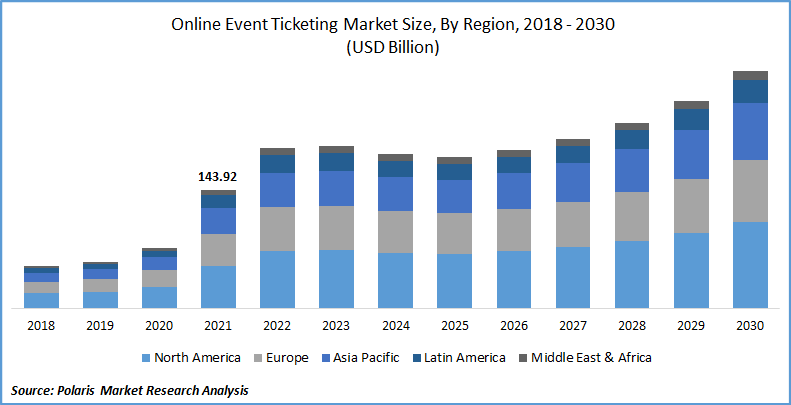
\includegraphics[width=\textwidth]{\FIGDIR/polaris-market-research}
    \source[\citeauthor{online_ticketing_polaris_market_research}]{}
    \label{fig:polaris-market-research}
\end{figure}

Avšak s rapidním vývojem v oblasti webových technologií je důležité sledovat a využívat nové trendy a technologie a přizpůsobovat jim takováto řešení, aby byla pro zákazníky stále atraktivní a relevantní.
Tato práce se proto zaměřuje na vývoj frontendové části webové aplikace prodeje vstupenek s rezervací míst, která bude využívat moderní webové technologie a nástroje, které jsou v současné době nejvíce využívané a oblíbené.
\pagebreak

%%% Sekce - Cíle práce
%%%%% Wording: ✅
%%%%% Styling: ✅
%%%%% References: ✅
%%%%% Grammar: ✅
%%% --------------------------------------------------------------
\section*{Cíle práce}
\addcontentsline{toc}{section}{Cíle práce}
\label{sec:uvod-cile-prace}
Cílem této práce je vyvinout prototyp responzivní webové aplikace nabízející prodej vstupenek s rezervací míst se zaměřením převážně na vývoj frontendové části.

Výsledkem této práce bude webová aplikace vyvinuta moderními webovými nástroji a technologiemi, která umožní potenciálním zákazníkům zobrazit mapu areálu nějaké akce či kulturní události, vybrat si jedno či více preferovaných míst, přidat si vstupenky do nákupního košíku a vytvořit tak objednávku.
Tato práce se bude zabývat vývojem takového webového řešení, ale pouze z pohledu frontendové části.
Ostatní funkčnosti, jako například backendový systém či administrační řešení, nebudou součástí této práce.

Nejprve bude ale pro vývoj třeba prozkoumat a analyzovat existující řešení prodeje vstupenek s rezervací míst, které jsou v současné době využívány.
Na základě identifikace klíčových částí takovýchto systémů budou následně vytvořeny dílčí uživatelské příběhy aplikace, které budou sloužit jako základ pro návrh uživatelského rozhraní.

Aby byla práce považována za úspěšně dokončenou, musí být splněny následující cíle:

\begin{itemize}
    \item Byly identifikovány klíčové prvky a funkčnosti webových řešení prodeje vstupenek s rezervací míst.
    \item Byl vytvořen návrh uživatelského rozhraní aplikace na základě definovaných uživatelských příběhů.
    \item Byla vyvinuta responzivní webová aplikace prodeje vstupenek s rezervací míst.
    \item Byla aplikace nasazena do produkčního prostředí.
\end{itemize}

% TODO: doplnit kapitoly
    \chapter{Praktická část}

Praktická část pojednává o~vývoji prototypu frontendu webové aplikace pro prodej vstupenek s~důrazem na implementaci funkčnosti rezervace míst. Nutno podotknout že výsledný prototyp nebude a ani není v plánu, aby byl plně funkční, nýbrž pouze ukazuje možnou implementaci konrkétních zvolených částí.\\

K implementaci prototypu je důležité předem vydefinovat jasnou specifikaci a požadavky na výsledný produkt. Bez těchto speicifkací by nebylo možné finální výsledek objektivně zhodnotit. Po jasné specifiaci požadavků bude potřeba prototyp vizuálně navrhnout a připravit jako podklad k implementaci. K té bude také třeba zanalyzovat konkrétní požadavky a zvolit správné technologie. Tento prototyp bude realizován pouze z frontendové části, tedy z pohledu vizuálního rozhraní pro potenciálního zákazníka, který si bude chtít zakoupit vstupenku s využitím rezervace místa. Z tohoto důvodu bude alespoň minimálně popsána funkčnost dostupného backednového rozhraní, který bude sloužit jako zdroj dat pro frontend.\\

Všechny zmíněné postupy budou v této části práce blíže popsány a vysvětleny v jednotlivých kapitolách.

\section{Specifikace a požadavky}
\label{sec:specifikace}
TODO

\section{Vizuální návrh}
\label{sec:navrh}
TODO

\section{Výběr technologií}
\label{sec:technologie}
TODO


%%% TODO: seznam použité literatury
%%% Reference se hledají v souboru priklady_literatury.bib. Aby se
%%% vytvořil seznam literatury, je třeba ocitovat alespoň jednu
%%% referenci, zkompilovat tento soubor latexem, pak bibtexem a znovu
%%% latexem. Tím se vytvoří seznam použitých referencí
%%% (BcPrace.bbl) a vloží se do práce na místě, kde se nachází příkaz
%%% \bibliography, tedy sem.
    \bibliography{main}
%%% seznam obrázků
    \listoffigures
%%% seznam tabulek
    \listoftables

%%% TODO
%%% Použité zkratky v bakalářské práci, včetně jejich vysvětlení.
    \chapter*{Seznam použitých zkratek}
    \addcontentsline{toc}{chapter}{Seznam použitých zkratek}
    \begin{description}
        \item[API] Application Programming Interface
        \item[SVG] Scalable Vector Graphics
        \item[HTML] HyperText Markup Language
    \end{description}

%%% TODO
%%% Přílohy k bakalářské práci, existují-li (různé dodatky jako výpisy programů,
%%% diagramy apod.). Každá příloha musí být alespoň jednou odkazována z vlastního
%%% textu práce. Přílohy se číslují.
    \chapter*{Přílohy}
    \addcontentsline{toc}{chapter}{Přílohy}


\end{document}
